\documentclass[journal,12pt,twocolumn]{IEEEtran}

\usepackage{setspace}
\usepackage{gensymb}
\singlespacing
\usepackage[cmex10]{amsmath}
\usepackage{amssymb}
\usepackage{xurl}

\usepackage{amsthm}
\usepackage{comment}
\usepackage{mathrsfs}
\usepackage{txfonts}
\usepackage{stfloats}
\usepackage{bm}
\usepackage{cite}
\usepackage{cases}
\usepackage{subfig}

\usepackage{longtable}
\usepackage{multirow}

\usepackage{enumitem}
\usepackage{mathtools}
\usepackage{steinmetz}
\usepackage{tikz}
\usepackage{circuitikz}
\usepackage{verbatim}
\usepackage{tfrupee}
\usepackage[breaklinks=true]{hyperref}
\usepackage{graphicx}
\usepackage{tkz-euclide}

\usetikzlibrary{calc,math}
\usepackage{listings}
    \usepackage{color}                                            %%
    \usepackage{array}                                            %%
    \usepackage{longtable}                                        %%
    \usepackage{calc}                                             %%
    \usepackage{multirow}                                         %%
    \usepackage{hhline}                                           %%
    \usepackage{ifthen}                                           %%
    \usepackage{lscape}     
\usepackage{multicol}
\usepackage{chngcntr}

\DeclareMathOperator*{\Res}{Res}

\renewcommand\thesection{\arabic{section}}
\renewcommand\thesubsection{\thesection.\arabic{subsection}}
\renewcommand\thesubsubsection{\thesubsection.\arabic{subsubsection}}

\renewcommand\thesectiondis{\arabic{section}}
\renewcommand\thesubsectiondis{\thesectiondis.\arabic{subsection}}
\renewcommand\thesubsubsectiondis{\thesubsectiondis.\arabic{subsubsection}}


\hyphenation{op-tical net-works semi-conduc-tor}
\def\inputGnumericTable{}                                 %%

\lstset{
%language=C,
frame=single, 
breaklines=true,
columns=fullflexible
}
\begin{document}


\newtheorem{theorem}{Theorem}[section]
\newtheorem{problem}{Problem}
\newtheorem{proposition}{Proposition}[section]
\newtheorem{lemma}{Lemma}[section]
\newtheorem{corollary}[theorem]{Corollary}
\newtheorem{example}{Example}[section]
\newtheorem{definition}[problem]{Definition}

\newcommand{\BEQA}{\begin{eqnarray}}
\newcommand{\EEQA}{\end{eqnarray}}
\newcommand{\define}{\stackrel{\triangle}{=}}
\bibliographystyle{IEEEtran}
\raggedbottom
\setlength{\parindent}{0pt}
\providecommand{\mbf}{\mathbf}
\providecommand{\pr}[1]{\ensuremath{\Pr\left(#1\right)}}
\providecommand{\qfunc}[1]{\ensuremath{Q\left(#1\right)}}
\providecommand{\sbrak}[1]{\ensuremath{{}\left[#1\right]}}
\providecommand{\lsbrak}[1]{\ensuremath{{}\left[#1\right.}}
\providecommand{\rsbrak}[1]{\ensuremath{{}\left.#1\right]}}
\providecommand{\brak}[1]{\ensuremath{\left(#1\right)}}
\providecommand{\lbrak}[1]{\ensuremath{\left(#1\right.}}
\providecommand{\rbrak}[1]{\ensuremath{\left.#1\right)}}
\providecommand{\cbrak}[1]{\ensuremath{\left\{#1\right\}}}
\providecommand{\lcbrak}[1]{\ensuremath{\left\{#1\right.}}
\providecommand{\rcbrak}[1]{\ensuremath{\left.#1\right\}}}
\theoremstyle{remark}
\newtheorem{rem}{Remark}
\newcommand{\sgn}{\mathop{\mathrm{sgn}}}
\providecommand{\abs}[1]{\vert#1\vert}
\providecommand{\res}[1]{\Res\displaylimits_{#1}} 
\providecommand{\norm}[1]{\lVert#1\rVert}
%\providecommand{\norm}[1]{\lVert#1\rVert}
\providecommand{\mtx}[1]{\mathbf{#1}}
\providecommand{\mean}[1]{E[ #1 ]}
\providecommand{\fourier}{\overset{\mathcal{F}}{ \rightleftharpoons}}
%\providecommand{\hilbert}{\overset{\mathcal{H}}{ \rightleftharpoons}}
\providecommand{\system}{\overset{\mathcal{H}}{ \longleftrightarrow}}
	%\newcommand{\solution}[2]{\textbf{Solution:}{#1}}
\newcommand{\solution}{\noindent \textbf{Solution: }}
\newcommand{\cosec}{\,\text{cosec}\,}
\providecommand{\dec}[2]{\ensuremath{\overset{#1}{\underset{#2}{\gtrless}}}}
\newcommand{\myvec}[1]{\ensuremath{\begin{pmatrix}#1\end{pmatrix}}}
\newcommand{\mydet}[1]{\ensuremath{\begin{vmatrix}#1\end{vmatrix}}}
\numberwithin{equation}{subsection}
\makeatletter
\@addtoreset{figure}{problem}
\makeatother
\let\StandardTheFigure\thefigure
\let\vec\mathbf
\renewcommand{\thefigure}{\theproblem}
\def\putbox#1#2#3{\makebox[0in][l]{\makebox[#1][l]{}\raisebox{\baselineskip}[0in][0in]{\raisebox{#2}[0in][0in]{#3}}}}
     \def\rightbox#1{\makebox[0in][r]{#1}}
     \def\centbox#1{\makebox[0in]{#1}}
     \def\topbox#1{\raisebox{-\baselineskip}[0in][0in]{#1}}
     \def\midbox#1{\raisebox{-0.5\baselineskip}[0in][0in]{#1}}
\vspace{3cm}
\title{AI1103 : Assignment 3}
\author{Prashanth Sriram S - CS20BTECH11039}
\maketitle
\newpage
\bigskip
\renewcommand{\thefigure}{\theenumi}
\renewcommand{\thetable}{\theenumi}
Download all python codes from 
\begin{lstlisting}
https://github.com/prashanthsriram-s/AI1103/tree/main/Assignment3/codes/
\end{lstlisting}
%
and latex codes from 
%
\begin{lstlisting}
https://github.com/prashanthsriram-s/AI1103/tree/main/Assignment3/Assignment3.tex
\end{lstlisting}
\section*{\textbf{Problem statement}}
(AS3)=UGC / MATH (mathA June 2017), Q.118
Suppose the random varible $X$ has the following probability density function
\begin{align}
f(x)=
\begin{cases}
\alpha(x-\mu)^{\alpha-1}e^{-(x-\mu)^\alpha} &x>\mu\\
0 &x\leq\mu,
\end{cases}
\end{align}
Where $\alpha>0, -\infty<\mu<\infty$. Which of the following statements are correct? The Hazard function of $X$ is\\
(A)an increasing function for all $\alpha>0$\\
(B) a decreasing function for all $\alpha>0$\\
(C)an increasing function for some $\alpha>0$\\
(D) a decreasing function for some $\alpha>0$
\section*{\textbf{Solution}}
The Hazard function of $X$,
\begin{align}
\lambda(X) = \frac{f(x)}{S(x)} \label{eq:1}
\end{align}
where $S(x)$ is the survival function given by,
\begin{align}
S(x) = P(X \geq x) = 1-F(x) = \int_{x}^{\infty}f(t)dt
\end{align}
\begin{lemma}
\begin{align}
S(x)=
\begin{cases}
e^{-(x-\mu)^\alpha} &x>\mu\\
1 &x\leq\mu
\end{cases}
\end{align}
\end{lemma}
\begin{proof}

\begin{align}
\int f(t)dt=\int \alpha(t-\mu)^{\alpha-1}e^{-(t-\mu)^\alpha}dt\\
=-e^{-(t-\mu)^\alpha} + C
\end{align}
If $x>\mu$, 
\begin{align}
S(x) = \int_{x}^{\infty} \alpha(t-\mu)^{\alpha-1}e^{-(t-\mu)^\alpha}dt\\
=-e^{-(t-\mu)^\alpha}]_{x}^{\infty}\\
=e^{-(x-\mu)^{\alpha}} \label{eq:2}
\end{align}
If $x\leq\mu$,
\begin{align}
S(x) = \int_{x}^{\mu}f(t)dt + \int_{\mu}^{\infty}f(t)dt\\
     = 0 + e^{-(\mu-\mu)^{\alpha}}\\
     =1 \label{eq:3}
\end{align}
From \eqref{eq:2} and \eqref{eq:3}, we get $S(x)$ as,
\begin{align}
S(x)=
\begin{cases}
e^{-(x-\mu)^\alpha} &x>\mu\\
1 &x\leq\mu \label{eq:4}
\end{cases}
\end{align}
\end{proof}
From \eqref{eq:1} and \eqref{eq:4}, we get
\begin{align}
\lambda(x) = 
\begin{cases}
\alpha(x-\mu)^{\alpha-1} &x>\mu\\
0 &x\leq\mu \label{eq:5}
\end{cases}
\end{align}
So,\\ if $\alpha>1$, $\lambda(x)$ is an increasing function
\begin{figure}[htp]
    \centering
    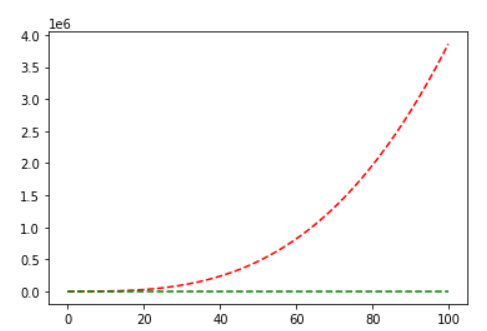
\includegraphics[width=8cm]{alphagrt1.png}
    \caption{$\alpha=2$ for red. $\alpha=1$ for green, $\mu=1$ for both}
    \label{fig:grt1}
\end{figure}
and\\ if $0<\alpha<1$, $\lambda(x)$ is a decreasing function
\begin{figure}[htp]
    \centering
    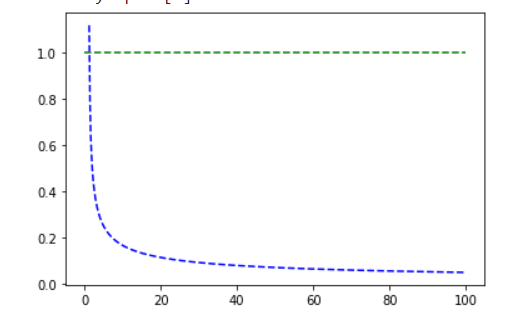
\includegraphics[width=8cm]{alphales1.png}
    \caption{$\alpha=0.5$ for blue. $\alpha=1$ for green, $\mu=1$ for both}
    \label{fig:les1}
\end{figure}
and\\ for $\alpha=1$, $\lambda(x)=1$, a constant function.\\
So, for some values of $\alpha$, it is increasing, for some it is decreasing function\\
\textbf{Therefore, answer is (C) and (D)}
\end{document}